\documentclass[a4paper]{scrreprt}
\usepackage{fullpage} % Slightly more margins
\usepackage{amsfonts}
\usepackage{fancyhdr}
\pagestyle{fancy}
\usepackage[english]{babel}
\selectlanguage{english}
\usepackage[utf8]{inputenc}
\usepackage{graphicx}
\usepackage{url}
\usepackage{textcomp}
\usepackage{amsmath}
\usepackage{lastpage}
\usepackage{pgf}
\usepackage{wrapfig}
\usepackage{fancyvrb}
\usepackage{courier}

% Create header and footer
\headheight 27pt
\pagestyle{fancyplain}
\lhead{\footnotesize{Object-Oriented Design, IV1350}}
\chead{}
\rhead{\footnotesize{Assignment 1 Report}}
\lfoot{}
\cfoot{\thepage  (\pageref{LastPage})}

% Create title page
\title{Assignment 1}
\subtitle{Object-Oriented Design, IV1350}
\author{Emil Tullstedt emiltu@kth.se}
\date{2014-05-19}

\graphicspath{ {./images/} }

\begin{document}

\maketitle

\tableofcontents %Generates the TOC

\chapter{Introduction}
This report describes an analyze of the requirements for a cache layout and the process of modeling the analyze as a domain model and a system sequence diagram. The report is made for the course \textit{IV1350} at KTH and is not made for usage in production.

\begin{small}
While analyzing the application, I co-operated with \textit{Martin Alge}, \textit{Jesper Falk} and \textit{Erik Pettersson}.
\end{small}

\chapter{Method}

There's a rather important difference between object-oriented design and object-oriented programming, similarly to the difference in the architect's process of designing a house and the artisan's process of building it.

The process of building a house is similar to the process of building software. For an artisan building a tree-house or raising a tent there's no need for a formal analysis, just as how simple applications and scripts often \textit{just happen} for a programmer.

Whenever you're building anything slightly more advanced, ranging from a playhouse to a chateau - you probably want to do an analysis and a design before actually constructing. The artisan will probably find herself to be insufficiently experienced for building a chateau, and will almost certainly fail if she were to start building by herself. Just as any programmer almost certainly will fail trying to build anything as complicated as an usable operating system or word processor as a hobby project\footnote{Obviously, if the artisan happened to be Linus Torvalds, the artisan would find a bunch of friends and they would together build the grandest and most beautiful chateau, but that's quite a bit off topic.}.

If the artisan were to try and construct a cottage, she would probably not need to consult an expert in the same way as the artisan would need to consult an expert in the process of building the chateau, but she would still have to spend quite a bit of time analyzing and designing the various plans for the cottage.

At the end of the day the process for doing any work which requires attention to both lots of details and the entirety is very much alike. Thus the artisan and the programmer has the same problems when facing a seemingly overwhelming project, and before implementation of the plans, all artists needs to consider the following:

\begin{enumerate}
\item What is the purpose of this project? (Analyzing)
\item What is needed to fill that purpose? (Designing)
\end{enumerate}

This report briefly covers the process of a programmer analyzing a smaller software project following an object-oriented analysis and design formula using UML.

\section{Domain Model}
\label{sec:domainmodel}
The very first step when analyzing a problem you've been tasked with solving programmatically would be to observe the nouns in the problem. When programming using the object-oriented paradigm, this is similar to the architects need of identifying what rooms to build and what furniture to place in each room. At this point the size of the bed doesn't really matter and it doesn't really matter if the kitchen has an inductive or a gas stove.

The purpose of the domain model in object-oriented analysis is to standardize the pattern of how a programmer shall scribble down the identified objects, much like how drawings have been standardized for engineers in general. This allows for a software architect to draw a domain model and then hand it over to a software implementer or a customer, and no matter which software architect have made the domain model, the customer or implementer should immediately be able to understand the model given that they are already accustomed to domain models.


\chapter{Result}
\label{sec:result}

\section{Domain Model: DataCache}
\label{sec:datacachedomainmodel}

When designing the domain model for the data cache (visible in fig. \ref{fig:domainmodel}) the key nouns identified were:

\begin{itemize}
\item User
\item Nickname
\item Program
\item Block Size
\item Block Count
\item Associativity
\item Cache Layout
\item Address Layout
\item Address Tag
\item Index
\item Offset
\item Cache
\item Instruction
\item Load
\item Store
\item Main Memory
\item Rows
\item Simulation data
\end{itemize}

When designing the domain model from this set of nouns it's important to embrace the idea that not all of these are actually conceptual classes in their own rights, for example, one can see that the \textit{Cache Layout} is defined as a coalition of \textit{Block Size}, \textit{Block Count} and \textit{Associativity}, just as the \textit{Address Layout} is a coalition of the \textit{Address Tag}, \textit{Index} and \textit{Offset}.

Based on this, you can build a category list where you set the nouns in different categories.

\begin{center}
	\begin{tabular}{| l | l |}
	\hline
	\textit{Category} & \textit{Content}
	\\ \hline
	\textbf{Actors} & Program, User
	\\ \hline
	\textbf{Containers} & Data Cache, Simulation Data, Main Memory, Rows
	\\ \hline
	\textbf{Contained items} & Rows, Nickname, Address Tag
	\\ \hline
	\textbf{Operations} & Instructions
	\\ \hline
	\textbf{Operation Types} & Load, Store
	\\ \hline
	\textbf{Layouts} & Cache Layout, Address Layout
	\\ \hline
	\textbf{Layout Properties} & Associativity, Block Size, Block Count, Address Tag, Index, Offset\\
	\hline
	\end{tabular}
\end{center}

With the category list in place the process of eliminating nouns from being conceptual classes in the domain model begins. When doing so, first place everything that logically will be a conceptual class of it's own in the domain model to begin with, and then try to find how these correlates with each other. Objects that are of simple data types and only contained and doesn't have any calculations of it's own are quickly inserted as attributes of other objects, such as everything I put in the layout property category is the attribute of a layout-object (unsurprisingly). Iterate this process a few times, find connections and try to eliminate as many conceptual classes as possible without having objects that feels like huge monoliths.

There's a few choices made during this process in the domain model visible in fig. \ref{fig:domainmodel} that's worth highlighting, namely:

\begin{itemize}
\item The \texttt{Program} conceptual class is unnecessary, as it is simply a container for the entire execution of the application. The \texttt{System} in the system sequence diagram fig. \ref{fig:ssd} is roughly equivalent to this conceptual class
\item The \texttt{Row} conceptual class is both a container and a contained object, and exists mostly because the instructions clearly says the \texttt{DataCache} may contain multiple locations
\item The \texttt{Cache Layout} and \texttt{Address Layout} might be interesting to merge. However, there's quite a few operations relating to either of them there's a risk that including both within the same conceptual class will create a monolithic giant conceptual class
\item The \texttt{Storage} conceptual class is based on the \texttt{Simulation Data} noun and the verb that requires the program to \textit{store} key execution data
\item The \texttt{User} conceptual class is the actor which operates on the program. The choice of storing nickname in the \texttt{Storage} conceptual class instead of within the user is because the user isn't conceptually seen as part of the actual programmable program, but as an external actor
\end{itemize}

\begin{figure}[h]
  \begin{center}
    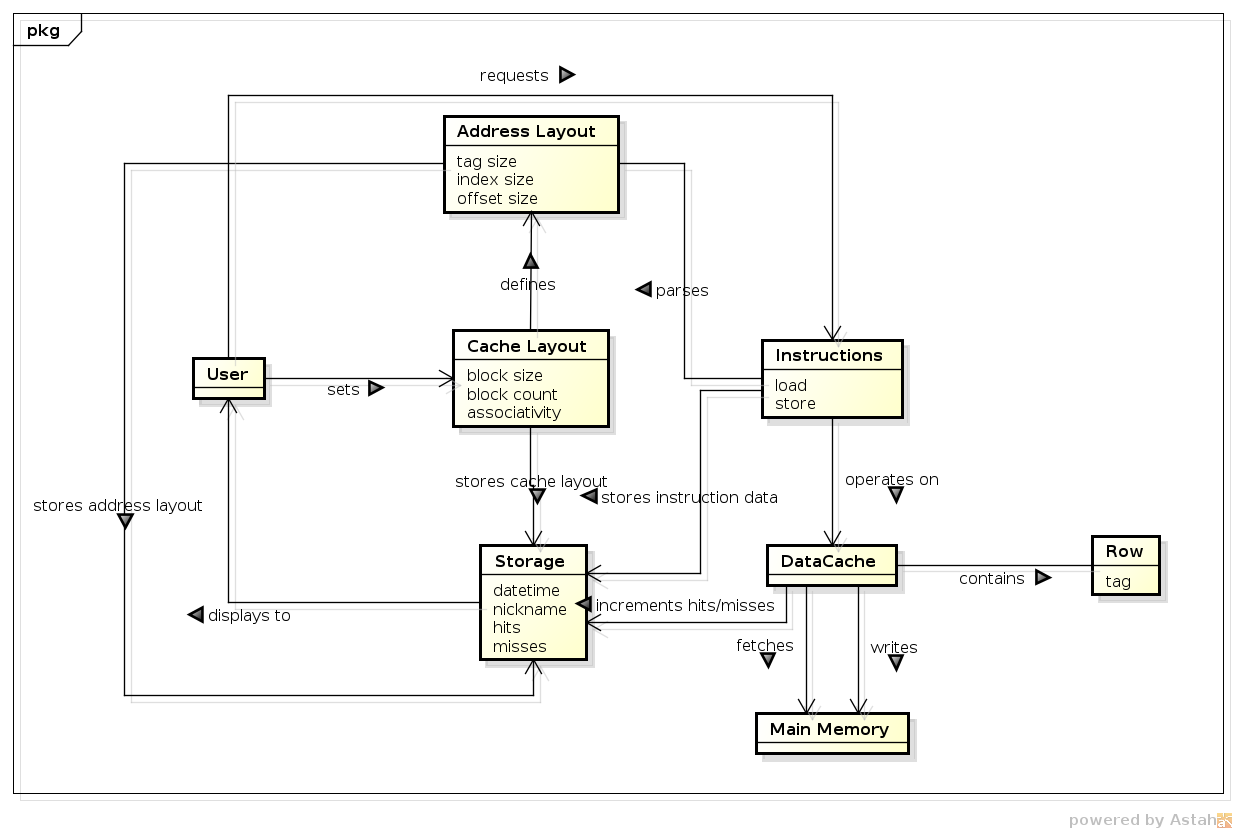
\includegraphics[scale=.5]{DomainModel.png}
    \caption{Domain model for the analyze of a data cache specified in the instructions which were made following the instructions in section \ref{sec:datacachedomainmodel}}
    \label{fig:domainmodel}
  \end{center}
\end{figure}

\newpage

\section{System Sequence Diagram: DataCache}

\begin{figure}[h]
  \begin{center}
    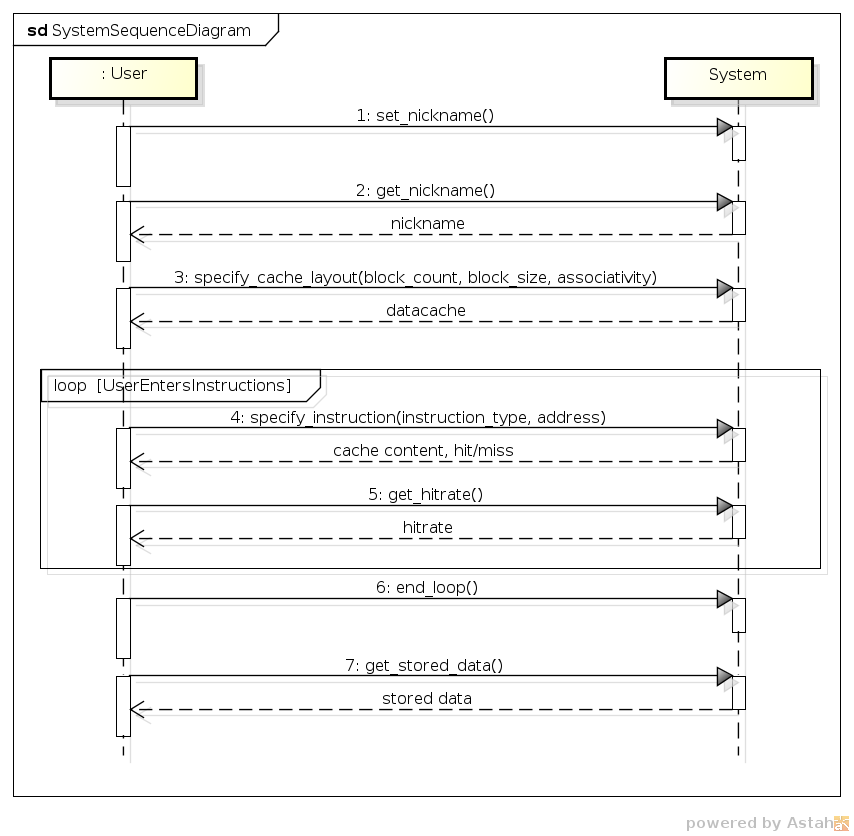
\includegraphics[scale=.7]{SystemSequenceDiagram.png}
    \caption{System Sequence Diagram for the data cache}
    \label{fig:ssd}
  \end{center}
\end{figure}
\end{document}